\documentclass{standalone}

\usepackage{tikz}
\usepackage{circuitikz}

\tikzset{block/.style = {draw, fill=white, very thick, rectangle, minimum height=1cm, minimum width=2cm},
         lblock/.style={draw,fill=white,very thick, rectangle, minimum height=3cm, minimum width=1cm},
         sum/.style= {draw, fill=white, very thick, circle, node distance=0.5cm}}

         
\begin{document}
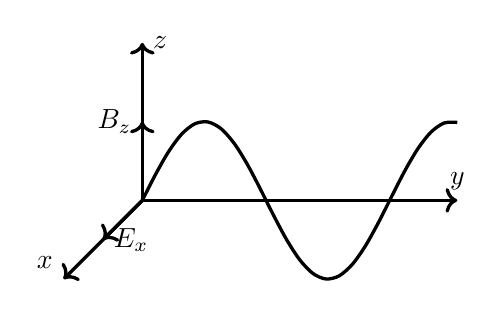
\begin{tikzpicture}[scale=2]
    \draw[->,very thick](0,0)--(2,0)node[above]{$y$};
    \draw[->,very thick](0,0)--(0,1)node[right]{$z$};
    \draw[->,very thick](0,0)--(-0.5,-0.5)node[above left]{$x$};

    \draw[->,very thick](0,0)--(0,0.5)node[left]{$B_z$};
    \draw[->,very thick](0,0)--(-0.25,-0.25)node[right]{$E_x$};
    \draw[-,very thick]plot[smooth, domain=0:2](\x,{0.5*sin(4*\x r)});
\end{tikzpicture}
\end{document}